% Options for packages loaded elsewhere
\PassOptionsToPackage{unicode}{hyperref}
\PassOptionsToPackage{hyphens}{url}
%
\documentclass[
]{article}
\usepackage{amsmath,amssymb}
\usepackage{lmodern}
\usepackage{iftex}
\ifPDFTeX
  \usepackage[T1]{fontenc}
  \usepackage[utf8]{inputenc}
  \usepackage{textcomp} % provide euro and other symbols
\else % if luatex or xetex
  \usepackage{unicode-math}
  \defaultfontfeatures{Scale=MatchLowercase}
  \defaultfontfeatures[\rmfamily]{Ligatures=TeX,Scale=1}
\fi
% Use upquote if available, for straight quotes in verbatim environments
\IfFileExists{upquote.sty}{\usepackage{upquote}}{}
\IfFileExists{microtype.sty}{% use microtype if available
  \usepackage[]{microtype}
  \UseMicrotypeSet[protrusion]{basicmath} % disable protrusion for tt fonts
}{}
\makeatletter
\@ifundefined{KOMAClassName}{% if non-KOMA class
  \IfFileExists{parskip.sty}{%
    \usepackage{parskip}
  }{% else
    \setlength{\parindent}{0pt}
    \setlength{\parskip}{6pt plus 2pt minus 1pt}}
}{% if KOMA class
  \KOMAoptions{parskip=half}}
\makeatother
\usepackage{xcolor}
\usepackage[margin=1in]{geometry}
\usepackage{longtable,booktabs,array}
\usepackage{calc} % for calculating minipage widths
% Correct order of tables after \paragraph or \subparagraph
\usepackage{etoolbox}
\makeatletter
\patchcmd\longtable{\par}{\if@noskipsec\mbox{}\fi\par}{}{}
\makeatother
% Allow footnotes in longtable head/foot
\IfFileExists{footnotehyper.sty}{\usepackage{footnotehyper}}{\usepackage{footnote}}
\makesavenoteenv{longtable}
\usepackage{graphicx}
\makeatletter
\def\maxwidth{\ifdim\Gin@nat@width>\linewidth\linewidth\else\Gin@nat@width\fi}
\def\maxheight{\ifdim\Gin@nat@height>\textheight\textheight\else\Gin@nat@height\fi}
\makeatother
% Scale images if necessary, so that they will not overflow the page
% margins by default, and it is still possible to overwrite the defaults
% using explicit options in \includegraphics[width, height, ...]{}
\setkeys{Gin}{width=\maxwidth,height=\maxheight,keepaspectratio}
% Set default figure placement to htbp
\makeatletter
\def\fps@figure{htbp}
\makeatother
\setlength{\emergencystretch}{3em} % prevent overfull lines
\providecommand{\tightlist}{%
  \setlength{\itemsep}{0pt}\setlength{\parskip}{0pt}}
\setcounter{secnumdepth}{5}
\newlength{\cslhangindent}
\setlength{\cslhangindent}{1.5em}
\newlength{\csllabelwidth}
\setlength{\csllabelwidth}{3em}
\newlength{\cslentryspacingunit} % times entry-spacing
\setlength{\cslentryspacingunit}{\parskip}
\newenvironment{CSLReferences}[2] % #1 hanging-ident, #2 entry spacing
 {% don't indent paragraphs
  \setlength{\parindent}{0pt}
  % turn on hanging indent if param 1 is 1
  \ifodd #1
  \let\oldpar\par
  \def\par{\hangindent=\cslhangindent\oldpar}
  \fi
  % set entry spacing
  \setlength{\parskip}{#2\cslentryspacingunit}
 }%
 {}
\usepackage{calc}
\newcommand{\CSLBlock}[1]{#1\hfill\break}
\newcommand{\CSLLeftMargin}[1]{\parbox[t]{\csllabelwidth}{#1}}
\newcommand{\CSLRightInline}[1]{\parbox[t]{\linewidth - \csllabelwidth}{#1}\break}
\newcommand{\CSLIndent}[1]{\hspace{\cslhangindent}#1}
\ifLuaTeX
  \usepackage{selnolig}  % disable illegal ligatures
\fi
\IfFileExists{bookmark.sty}{\usepackage{bookmark}}{\usepackage{hyperref}}
\IfFileExists{xurl.sty}{\usepackage{xurl}}{} % add URL line breaks if available
\urlstyle{same} % disable monospaced font for URLs
\hypersetup{
  pdftitle={Different rules for binocular combination of luminance flicker in cortical and subcortical pathways},
  pdfauthor={Federico G. Segala, Aurelio Bruno, Myat T. Aung, Alex R. Wade \& Daniel H. Baker},
  hidelinks,
  pdfcreator={LaTeX via pandoc}}

\title{Different rules for binocular combination of luminance flicker in cortical and subcortical pathways}
\author{Federico G. Segala, Aurelio Bruno, Myat T. Aung, Alex R. Wade \& Daniel H. Baker}
\date{2022-10-16}

\begin{document}
\maketitle

\hypertarget{abstract}{%
\section{Abstract}\label{abstract}}

\hypertarget{introduction}{%
\section{Introduction}\label{introduction}}

\begin{center}\rule{0.5\linewidth}{0.5pt}\end{center}

OK, some pointers for the introduction:

I think we need to draw a distinction between binocular summation at threshold (on which there is a big literature) and binocular facilitation above threshold. Much of the introduction is focussed on threshold measures, but actually I think our focus here is more about suprathreshold conditions where we usually see little facilitation. I think it will help the reader if we use the term summation only to refer to threshold phenomena, and facilitation in the more general case (I've tried to do this elsewhere in the paper).

The key points should be:

\begin{enumerate}
\def\labelenumi{\arabic{enumi}.}
\item
  For grating stimuli, there are summation effects at threshold, but these are lost at high contrasts.
\item
  Binocular combination happens in multiple pathways, including the pupil pathway. (This is a good place to mention the Quaia paper).
\item
  We don't know much about the pupil response, though it is clearly binocular because of the consensual response (convergence and divergence seem to be other ways of saying the same thing, so not sure they are worth mentioning).
\item
  Actually there's not much work on temporal binocular combination even in the primary visual pathway.
\item
  We have developed a novel paradigm that allows us to probe both cortical and subcortical pathways simultaneously for flickering light.
\end{enumerate}

I wouldn't say too much about models, or about the matching experiment, at this stage.

\begin{center}\rule{0.5\linewidth}{0.5pt}\end{center}

Binocular combination provides a higher visual sensitivity than monocular viewing. This superiority is known as binocular summation and is defined by the binocular summation ratio (BSR), which was originally believed to be around \(\sqrt{2}\) (\(\approx1.4\)) for grating stimuli at detection threshold (Campbell and Green, 1965). In other words, a monocular stimulus can elicit the same response as a binocular stimulus if it has a contrast that is 1.4 times higher. This led Legge to develop a widely accepted explanation that used quadratic summation to describe binocular combination (Legge, 1984): monocular signals from the right (R) and the left (L) eyes are squared before being summed together and the binocular response (B) is given by the square root of the output (B = \(\sqrt{R^2 + L^2}\), when R and L are equal to 1, the output is \(\sqrt{2}\)). However, subsequent research has shown that these explanations are not fully adequate to account for binocular summation. Both of these accounts constitute single channel models, and this type of model has been shown to not being able to account for contrast detection in the presence of noise (Anderson and Movshon, 1989). Moreover, more recent research has shown that the summation ratio can vary greatly between \(\sqrt{2}\) and 2 depending on factors such as the spatial and temporal frequency of a stimulus or the sensitivity difference between the eyes (Baker et al., 2018). These observations led to the development of multistage gain control models, which combine binocular summation and interocular suppression, and can account for contrast matching, detection and discrimination for spatial contrast (Ding and Sperling, 2006; Meese et al., 2006).

In general, it seems that the mechanisms behind binocular combination have been thoroughly studied, as have been the anatomical pathways behind it: light enters the eye though the pupil and signals are sent from the left and right retinae to the primary visual cortex, remaining anatomically isolated while passing through the lateral geniculate nucleus (LGN) until they reach V1, where they are binocularly combined (Purves et al., 2008). However, there is an eye component that is often underestimated in its role to determine the quality of visual information: the pupil. The pupils are openings found in the centre of the eyes that appear to be black and allow light to enter the eyes. Their size determines how much light will reach the retina and it is usually determined by the ambient levels of light: in brightness the pupils will constrict and in darkness they will dilate. This is known as the pupillary light response (PLR). The anatomical pathways that regulate this response are well understood and are very clearly and extensively described in the literature (Angée et al., 2021; Mathôt, 2018; McDougal and Gamlin, 2010; Wang and Munoz, 2015). However, they are anatomically distinct from the LGN-V1 pathway meaning that binocular combination occurs separately in anatomically distinct pathways. Given this, not much is known about the computational processes behind the PLR except for some evidence of binocular interaction. The presence of a consensual response in one eye when the other is being stimulated, and the presence of convergence (one pupil responds to illumination in either retina) and divergence (both pupils respond to illumination of one retina) (Wyatt and Musselman, 1981) are evidence of this binocular interaction.

With this in mind we designed an experiment that simultaneously recorded electrophysiological and pupillometric responses to investigate the combination of flickering light signals in both the visual cortex and the pupils. The results should offer new insight about basic neural circuits and information on how they might be affected in clinical disorders of vision (e.g.~amblyopia). Based on previous literature, we expected to find a non-linear combination of the responses in visual cortex, as described by the gain control mechanisms, and a more linear combination of the responses and a greater binocular response at the level of the pupils.

Several models have been developed and proposed to describe binocular combination and contrast matching results for spatial contrast. Among these, the models proposed by Ding and Sperling (2006) and Meese and colleagues (2006) are widely accepted. These models incorporate a dynamic contrast gain control, which allows to develop a model that combines binocular summation and interocular suppression The first model is a multistage model that consists of two pairs of gain control mechanisms that inhibit each other (Ding and Sperling, 2006). In the earlier stage, the right and left eye channels exert gain control on the other channel. Then, they exert gain control on the other channel's gain control. Lastly, the outputs from each channel are summed binocularly to determine the binocular signal's magnitude. The second model is similar as it also incorporates gain control mechanisms (Meese et al., 2006). In the first stage, it is applied to the left and right eye channels with suppression from the other eye. Then the signal from the two eyes is summed binocularly and gain control is applied a second time. This second model in particular is interesting and relevant as it was designed to also explain data from matching experiments.

To follow up on the results that we obtained, we decided to perform a contrast matching experiment to investigate whether perception of flickering light is consistent with the results observed in the cortical pathways (visual cortex) or the subcortical pathways (pupils). Matching is a paradigm in which the perceived brightness of a standard stimulus is matched to that of a target stimulus. In the latter, the interocular ratios of luminance are varied to obtain an equibrightness curve. Previous literature has used this paradigm to investigate the binocular fusion of static stimuli and the temporal combination of spatial flickering of spatial increments (a bright target on a dark background) and decrements (a dark target on a bright background) (Anstis and Ho, 1998; Levelt, 1965). For spatial increments, it was found that binocular fusion seems to follow approximately linear combination rules. This means that, for a monocular stimulus to elicit the same response as a binocular stimulus, the former needs to have twice the signal of the latter. On the other hand, spatial decrements follow a winner-takes-all pattern. This means that the observer is seeing what the eye that is receiving the strongest signal is seeing.

Our experiment used different stimuli than the ones used by Anstis and Ho (1998): in the binocular fusion experiment, their stimuli were not flickering and, in the flicker experiment, they were always shown in both eyes. In our experiment, in some conditions, the flicker was shown to only one eye. Moreover, they were looking at the temporal fusion of the flicker while we focussed on the binocular fusion of the flicker. Based on this and on the results from our first experiment, we expected to find a near linear summation of the responses.

\hypertarget{methods}{%
\section{Methods}\label{methods}}

\hypertarget{participants}{%
\subsection{Participants}\label{participants}}

Thirty, twelve and ten participants were recruited for Experiments 1, 2 and 3 respectively. All participants had normal or corrected to normal binocular vision, and gave written informed consent.

\hypertarget{apparatus-stimuli}{%
\subsection{Apparatus \& stimuli}\label{apparatus-stimuli}}

The stimuli were two discs of flickering light with a diameter of 3.74 degrees, presented on a black background. The same stimuli were used for all three experiments. Four dark red lines were added around both discs to help with their fusion into one binocular disc (see insert in Figure \ref{fig:pupildata}b for an example of the fused stimulus). The discs were viewed through a four-mirror stereoscope, which used front silvered mirrors to avoid internal reflections, and meant that participants saw a single fused disc. The use of a stereoscope allowed us to modulate the stimuli in three different ocular configurations: monocular, binocular, and dichoptic. Note that during monocular presentation of flicker, the unstimulated eye still saw the static (non-flickering) disc of mean luminance.

All stimuli were displayed at a mean luminance of 42 cd/m\(^2\) on an Iiyama Vision Master™ Pro 510 display (800 x 600 pixels, 60 Hz refresh rate), which was gamma corrected using a Minolta LS-110 (Minolta Camera Co.~Ltd., Japan). For experiments 1 and 2, the stimuli were presented using Psychopy (v3.0.7). For experiment 3, the stimuli were presented using Psychopy (v2022.1.1).

EEG data were collected for Experiments 1 and 2 using a 64-electrode ANT WaveGuard cap and the signals were recorded at 1 kHz using the ASA software (ANT Neuro, Netherlands). Pupillometry data were collected for Experiment 1 using a binocular Pupil Core eye-tracker (Pupil Labs GmbH, Berlin, Germany; Kassner et al. (2014)) running at 120 Hz, and the signals were recorded with the Pupil Capture software.

\hypertarget{procedure}{%
\subsection{Procedure}\label{procedure}}

Before each experiment, participants calibrated the stereoscope by adjusting the angle of the mirrors. This was done so that they would perceive the two discs as one fused disc when looking at the screen through the stereoscope.

\hypertarget{experiment-1-simultaneous-eeg-and-pupillometry}{%
\subsubsection{Experiment 1: simultaneous EEG and pupillometry}\label{experiment-1-simultaneous-eeg-and-pupillometry}}

The experiment was conducted in a windowless room, in which the only light source was the monitor. The participants sat at 99 cm from the monitor and the total optical viewing distance (through the stereoscope) was 107 cm. The experiment was carried out in one session lasting 45 minutes in total, divided in three blocks of 15 minutes each. In each block, there were 60 trials in total lasting 15 seconds each (12s of stimulus presentation, with an interstimulus interval of 3s). The participants were given no specific task instructions, but were asked to look at the fixation crosses in the middle of the two discs while trying to minimise their blinking during the presentation period.
We included six distinct ocular conditions, each at five temporal target contrast levels (combined factorially) relative to the mean luminance: 6, 12, 24, 48 and 96\%. In the first three conditions, the discs flickered at 2 Hz, in either a monocular, binocular, or dichoptic arrangement. In the dichoptic condition the non-target eye saw a fixed luminance contrast of 48\%. In the remaining three conditions (termed the cross-frequency conditions) one eye's disc flickered at 1.6Hz, and the other eye's disc flickered at 2Hz. We also tested monocular (one eye sees 1.6Hz flicker, the other sees mean luminance), binocular (one eye sees each frequency at the target contrast) and dichoptic (target stimulus flickering at 2Hz, mask contrast of 48\% at 1.6Hz in the other eye) arrangements. The rationale for flickering both eyes at 2Hz is that we can then measure summation behaviour between the eyes in the pupil and EEG response at 2Hz. The rationale for flickering the eyes at different frequencies is that this permits measurement of suppression between the eyes (i.e.~the reduction in the 2Hz response when a 1.6Hz mask component is added to the other eye). We counterbalanced presentation of the target stimulus across the left and right eyes.

\hypertarget{experiment-2-eeg-responses-across-temporal-frequency}{%
\subsubsection{Experiment 2: EEG responses across temporal frequency}\label{experiment-2-eeg-responses-across-temporal-frequency}}

This experiment used the same equipment set up as Experiment 1, except that the eye tracker was not used. Unlike the first experiment, only one contrast level was used (96\%) and the discs were set to flicker at five different frequencies (2, 4, 8, 16 and 30 Hz). Only two ocular configurations, monocular and binocular, were used, with the latter having both discs flickering at the same frequency. The experiment was carried out in one session lasting 25 minutes in total, divided into five blocks of 5 minutes each. In each block, there were 20 trials in total with the same timing as for Experiment 1.

\hypertarget{experiment-3-temporal-contrast-matching}{%
\subsubsection{Experiment 3: temporal contrast matching}\label{experiment-3-temporal-contrast-matching}}

The experiment was conducted in a darkened room with a blacked-out window. The display equipment (monitor and stereoscope) were the same as for the two previous experiments, but no EEG or pupillometry data were collected. A two-interval contrast matching procedure was used to collect data. In one interval, participants were presented with a standard fused disc that flickered at a set contrast level (either 24 or 48\%), which was selected by the experimenter at the beginning of each block. In the other interval, a target disc flickering at varying contrast levels was displayed. The contrast level of the target was controlled by a 1-up, 1-down staircase moving in logarithmic (dB) steps of contrast. The ratio of flicker amplitudes in the left and right eyes was varied across blocks and was set to be 0, 0.25, 0.5, 0.75 or 1 (9 distinct conditions). The standard and target discs were displayed for 1 second each, with an interstimulus interval of 0.5 seconds. After the discs appeared on screen, the participants had to indicate which interval they perceived as having the more intense flicker. The intervals were randomly ordered, and all discs flickered at a frequency of 2 Hz (two cycles in sine phase).

Due to its long duration (approximately 3 hours in total), the participants completed the experiment across multiple sessions initiated at their own convenience The experiment was divided into 54 blocks (3 repetitions \(\times\) 2 standard contrasts \(\times\) 9 target ratios), which lasted on average 3 minutes each, depending on the response speed of the participant. In each block, there were a total of 50 trials. No auditory feedback was given for this subjective task.

\hypertarget{data-analysis}{%
\subsection{Data analysis}\label{data-analysis}}

EEG data were converted from the ANT-EEProbe format to a compressed csv text file using a custom Matlab script and components of the EEGlab toolbox (Delorme and Makeig, 2004). The data for each participant were then loaded into R for analysis where a ten-second waveform for each trial at each electrode was extracted (omitting the first two seconds). The fast Fourier transform was calculated for each waveform, and the spectrum stored in a matrix. All repetitions of each condition were then averaged for each electrode. They were then averaged across four occipital electrodes (\emph{POz}, \emph{Oz}, \emph{O1}, \emph{O2}), to obtain individual results. Finally, these were averaged across participants to obtain the group results. All averaging retained the phase information (i.e.~coherent averaging), and at each stage we excluded data points with a Mahalanobis distance exceeding \(D\) = 3 from the complex-valued mean (see Baker, 2021). For statistical comparisons of complex-valued data, we use the \(ANOVA^2_{circ}\) statistic described by Baker (2021). This is a multivariate extension of ANOVA that assumes equal variance of the real and imaginary Fourier components, or equivalently, an extension of the \(T^2_{circ}\) statistic of Victor and Mast (1991) that can compare more than two conditions.

A similar analysis pipeline was adopted for the pupillometry data. The data were converted from mp4 videos to a csv text file using the Pupil Player software (Kassner et al., 2014), which estimated pupil diameter for each eye on each frame using a 3D model of the eyeball. The individual data were then loaded into R for analysis, where again a ten-second waveform for each trial in each eye was extracted (excluding the first two seconds after stimulus onset). We interpolated across any dropped or missing frames to ensure regular and continuous sampling over time. The fast Fourier transform was calculated for each waveform, and all repetitions of each condition were pooled across eye and then averaged. Finally, data were averaged across all participants to obtain the group results. Again, we used coherent averaging, and excluded outlying data points in the same way as for the EEG data. Note that previous pupillometry studies using luminance flicker have tended to fit sine-waves to the data, rather than using Fourier analysis (e.g. Spitschan et al., 2014). Our novel approach is more robust to noise at other frequencies, and makes the pupillometry analysis consistent with standard practice in steady-state EEG analysis (e.g. Figueira et al., 2022)

To analyse the matching data, we pooled the trial responses across all repetitions of a given condition for each participant. We then fitted a cumulative normal psychometric function to estimate the point of subjective equality at the 50\% level. Thresholds were averaged across participants in logarithmic (dB) units. For all experiments, we used a bootstrapping procedure with 1000 iterations to estimate standard errors across participants. All analysis and figure construction was conducted using a single R-script, available online, making this study fully computationally reproducible.

\hypertarget{computational-model-and-parameter-estimation}{%
\subsection{Computational model and parameter estimation}\label{computational-model-and-parameter-estimation}}

To describe our data, we chose a model of binocular contrast gain control with the same general form as the first stage of the model proposed by Meese et al. (2006). The second gain control stage was omitted (consistent with Baker and Wade, 2017) to simplify the model and reduce the number of free parameters. The response of the left eye's channel is given by:

\begin{equation}
\label{eq:respL}
Resp_L = \frac{L^2}{Z + L + wR},
\end{equation}

with an equivalent expression for the right eye:

\begin{equation}
\label{eq:respR}
Resp_R = \frac{R^2}{Z + R + wL}.
\end{equation}

In both equations, \emph{L} and \emph{R} are the contrast signals from the left and right eyes, \emph{Z} is a saturation constant that shifts the contrast-response function laterally, and \emph{w} is the weight of suppression from the other eye.

The responses from the two eyes are then summed binocularly:

\begin{equation}
\label{eq:respB}
Resp_B = R_{max}(Resp_L + Resp_R) + n,
\end{equation}

where \emph{n} is a noise parameter, and \(R_{max}\) scales the overall response amplitude. The \(R_{max}\) parameter was omitted when modelling the contrast matching data, as it had no effect in this paradigm.

Despite being derived from the model proposed by Meese et al. (2006), the simplifications applied to this architecture make it very similar to other models (e.g. Ding and Sperling, 2006; Legge, 1984; Schrödinger, 1926). In particular we fixed the numerator exponent at 2 in our model, because otherwise this value tends to trade off with the weight of interocular suppression (see Baker et al., 2012; Kingdom and Libenson, 2015). Our key parameter of interest is the weight of interocular suppression. Large values around \(w\) = 1 result in a very small or nonexistent binocular advantage at suprathreshold contrasts, consistent with previous work using grating stimuli (Baker and Wade, 2017). Low values around \(w\) = 0 produce substantial, near-linear binocular facilitation (Baker et al., 2020).

We implemented the model within a Bayesian framework using the Stan software (Carpenter et al., 2017). This allowed us to estimate group-level posterior parameter distributions for the weight of interocular suppression, \(w\), and the other free model parameters \(R_{max}\), \(Z\) and \(n\). The prior distributions for all parameters were Gaussian, with means and standard deviations of 1 and 0.5 for \(w\) and \(R_{max}\), and 5 and 2 for \(Z\) and \(n\). We sampled from a Student's t-distribution for the amplitudes in the pupillometry and EEG experiments, and from a Bernoulli distribution for the single trial matching data. The models were fit using the individual data across all participants, independently for each data set. Because we used coherent averaging across participants, the group average amplitudes are shifted vertically relative to the model predictions, which are based on hierarchical fits to the individual participant amplitudes (put another way, the model does not implement coherent averaging). However it is clear that the character of the model in all cases gives a good representation of the data. We sampled over a million steps for each data set, using a computer cluster, and retained 10\% of samples for plotting.

\hypertarget{preregistration-data-and-code-availability}{%
\subsection{Preregistration, data and code availability}\label{preregistration-data-and-code-availability}}

We initially preregistered our main hypotheses and analysis intentions for the first experiment. We then conducted a pilot study with N=12 participants, before making some minor changes to the stimulus (we added dim red lines to aid binocular fusion). We then ran the main experiment, followed by two additional experiments that were not preregistered. The preregistration document, raw data files, and experimental and analysis code, are available on the project repository: \url{https://osf.io/tbema/}.

\hypertarget{results}{%
\section{Results}\label{results}}

\hypertarget{experiment-1}{%
\subsection{Experiment 1}\label{experiment-1}}

The pupillometry results are summarised in Figure \ref{fig:pupildata}. The group average waveform for binocular presentation is shown in Figure \ref{fig:pupildata}a. There is a substantial pupil constriction at stimulus onset, followed by visible oscillations at the flicker frequency (2Hz, see waveform at foot). The average Fourier spectrum is displayed in Figure \ref{fig:pupildata}b, and shows a substantial spike at 2 Hz, but no evidence of a second harmonic response at 4Hz. These results demonstrate that our paradigm can evoke measurable steady-state pupil responses at 2Hz.

\begin{figure}

{\centering 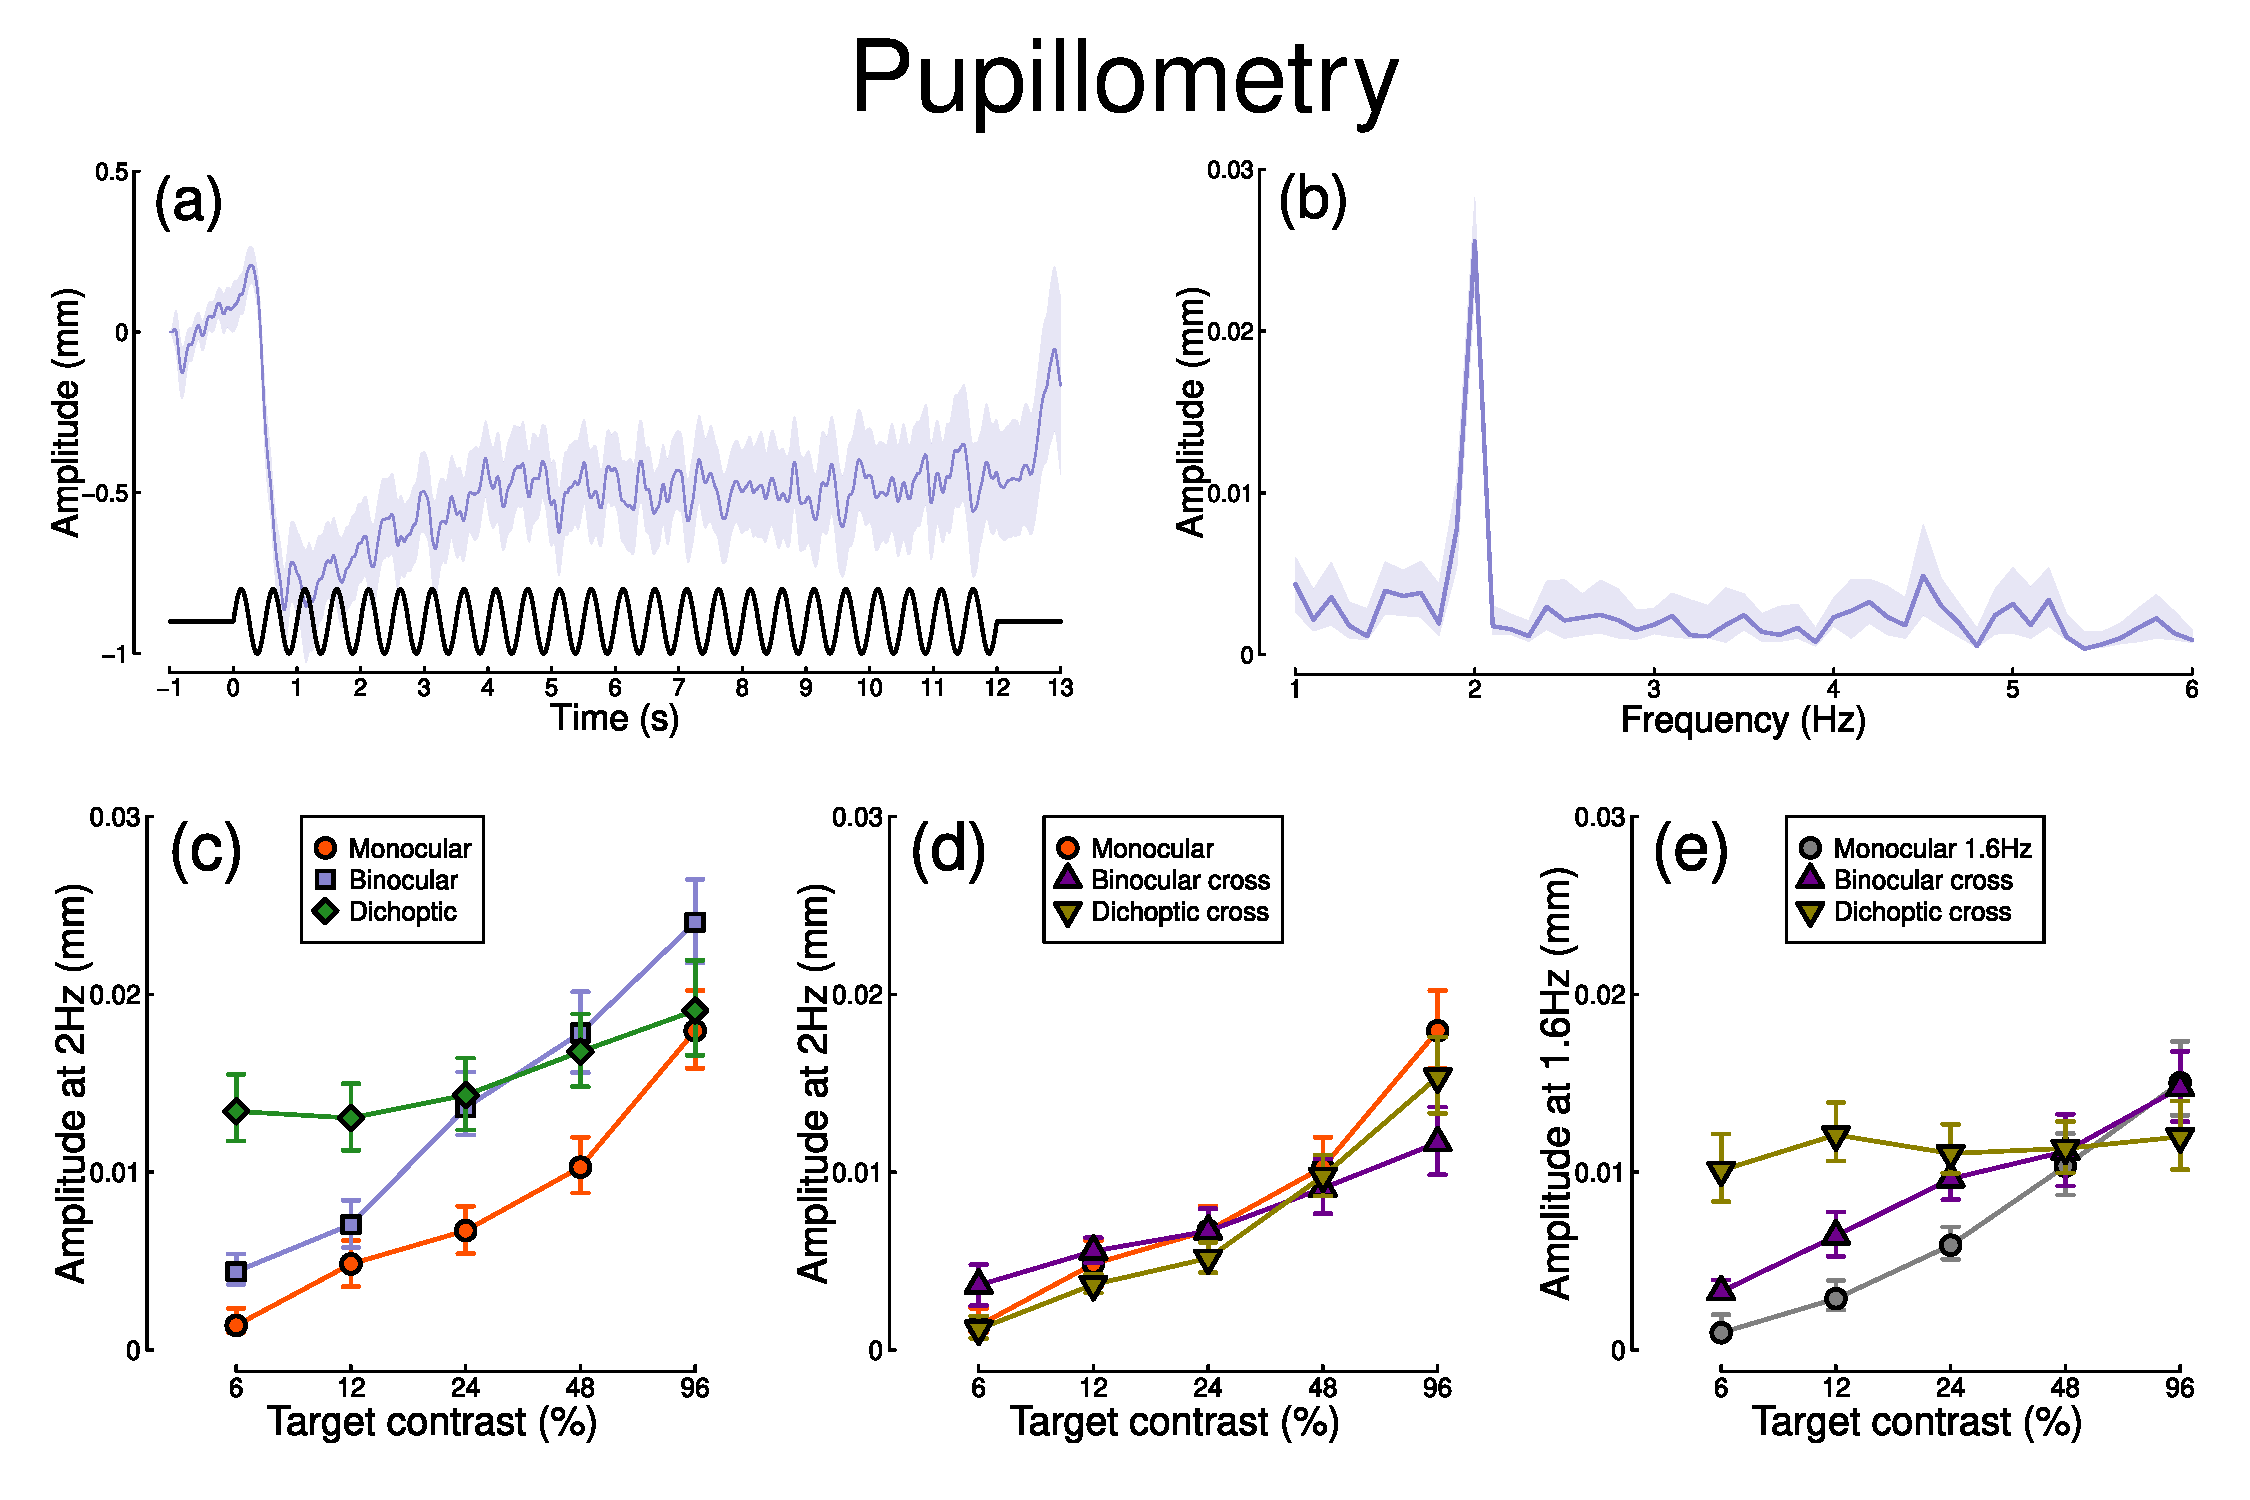
\includegraphics{Figures/pupildata} 

}

\caption{Summary of pupillometry results for N=30 participants. Panel (a) shows a group average waveform for binocular presentation (low pass filtered at 5Hz), with the driving signal plotted at the foot. Panel (b) shows the average Fourier spectrum, with an inset image illustrating the stimulus appearance (upper right). Panels (c,d) show contrast response functions at 2Hz for different conditions. Panel (e) shows contrast response functions at 1.6Hz for three conditions. Shaded regions and error bars indicate bootstrapped standard errors.}\label{fig:pupildata}
\end{figure}

Figure \ref{fig:pupildata}c shows contrast response functions in response to stimuli flickering only at 2Hz. Response amplitudes increased monotonically with target contrast, confirming that our paradigm is suitable for measuring contrast-dependent differences in response (to our knowledge this is the first time this has been demonstrated). The amplitude of the binocular condition (blue squares) is consistently greater than that of the monocular condition (red circles) across all target contrasts. A \(2\times5\) repeated measures \(ANOVA^2_{circ}\) (Baker, 2021) comparing these conditions revealed a significant main effect of target contrast (F(8,580) = 16.79, \(p\) \textless{} 0.001), a significant effect of condition (F(2,580) = 11.04, \(p\) \textless{} 0.001), and a significant interaction (F(8,580) = 56.25, \(p\) \textless{} 0.001). The dichoptic condition begins at a much higher amplitude, owing to binocular combination of the target and high (48\%) contrast mask, and then increases slightly with increasing target contrast (main effect of target contrast: F(8,232) = 3.03, \(p\) \textless{} 0.003).

In Figure \ref{fig:pupildata}d, we plot responses to monocular target stimuli flickering at 2Hz, when the other eye viewed stimuli flickering at 1.6Hz (the red monocular-only data are replotted from Figure \ref{fig:pupildata}c for comparison). When the 1.6Hz component had the same contrast as the target (the binocular cross condition, shown in purple) responses were facilitated slightly at low contrasts, and suppressed at the highest target contrasts (interaction between contrast and condition: F(8,580) = 52.94, \(p\) \textless{} 0.001). When the 1.6Hz component had a fixed contrast of 48\% (the dichoptic cross condition, shown in yellow), responses were suppressed slightly across the contrast range (interaction between contrast and condition: F(8,580) = 62.05, \(p\) \textless{} 0.001).

Figure \ref{fig:pupildata}e shows responses at 1.6Hz, for the same conditions, as well as for a condition in which a monocular stimulus flickered at 1.6Hz (grey circles). Surprisingly there appears to be a slight facilitation effect in the binocular cross condition, particularly at lower contrasts. The dichoptic cross condition does not show clear modulation with target contrast.

Figure \ref{fig:EEGdata} shows equivalent results, measured contemporaneously using EEG. Figure \ref{fig:EEGdata}a shows the group average waveform for binocular presentation, and Figure \ref{fig:EEGdata}b shows the Fourier spectrum for binocular presentation, both averaged across four posterior electrodes (\emph{Oz}, \emph{POz}, \emph{O1} and \emph{O2}, marked on the inset scalp plots). Unlike for the pupillometry data, there are clear responses at both the first harmonic frequency (2Hz), and also the second harmonic frequency (4Hz). We therefore calculated contrast response functions at both first and second harmonic frequencies.

\begin{figure}

{\centering 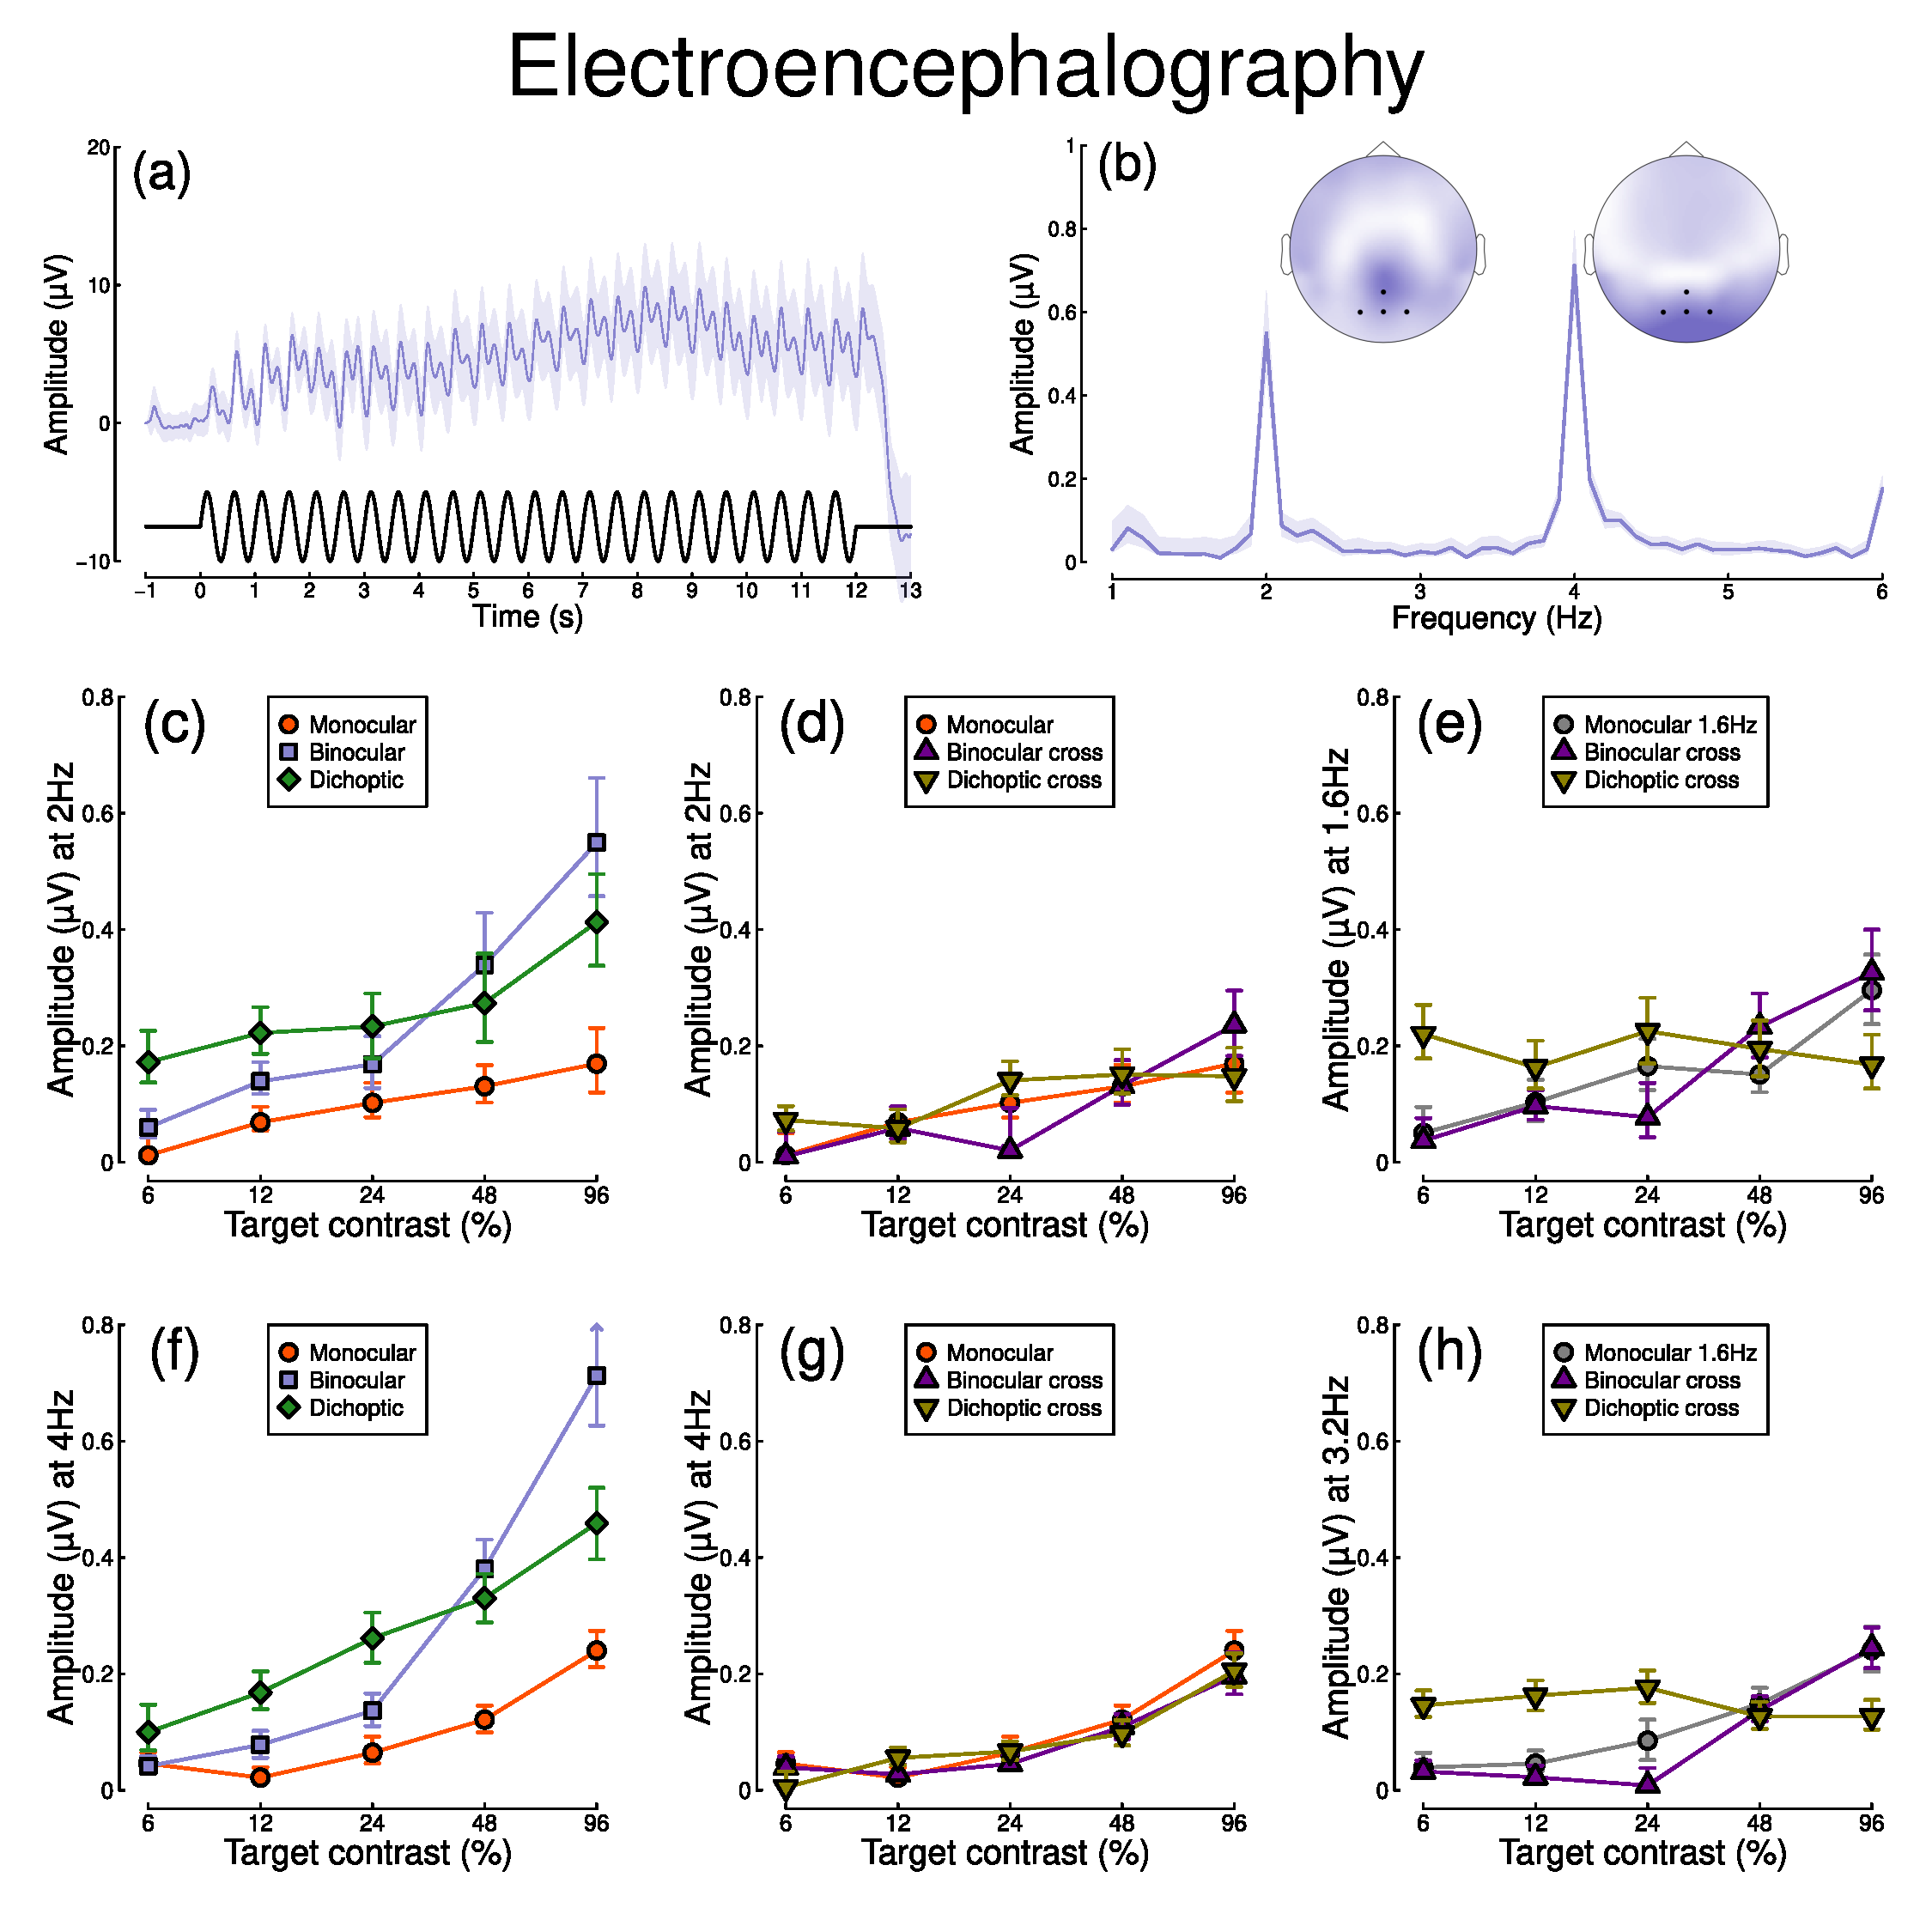
\includegraphics{Figures/EEGdata} 

}

\caption{Summary of EEG results for N=30 participants. Panel (a) shows a group average waveform for binocular presentation (low pass filtered at 5Hz), with the driving signal plotted at the foot. Panel (b) shows the average Fourier spectrum, and inset scalp distributions. Black dots on the scalp plots indicate electrodes Oz, POz, O1 and O2. Panels (c,d) show contrast response functions at 2Hz for different conditions. Panel (e) shows contrast response functions at 1.6Hz for three conditions. Panels (f-h) are in the same format but for the second harmonic responses. Shaded regions and error bars indicate bootstrapped standard errors.}\label{fig:EEGdata}
\end{figure}

When stimuli in both eyes flicker at 2Hz, the binocular responses at the first (Figure \ref{fig:EEGdata}c) and second (Figure \ref{fig:EEGdata}f) harmonics are substantially greater than the monocular responses, particularly at high contrasts. Analysis of variance on the complex values (\(ANOVA^2_{circ}\)) revealed a main effect of contrast (F(8,580) = 4.38, \(p\) \textless{} 0.001) and an interaction effect (F(8,580) = 61.58, \(p\) \textless{} 0.001), but no effect of condition (\(p\) = 0.13). For the cross-frequency conditions (Figure \ref{fig:EEGdata}d,g), there was no appreciable effect of adding a 1.6Hz component on the response at 2Hz or 4Hz (no effect of condition, and no interaction). Similarly, there were no clear interocular interactions between frequencies in the responses at 1.6Hz (Figure \ref{fig:EEGdata}e) and 3.2Hz (Figure \ref{fig:EEGdata}h). This pattern of results suggests that processing of temporal luminance modulations happens in a more linear way in visual cortex (indexed by EEG), compared with subcortical pathways (indexed by pupillometry), and shows no evidence of interocular suppression.

Finally, we calculated the ratio of binocular to monocular responses across the three data types from Experiment 1. Figure \ref{fig:BSratios} shows that these ratios are approximately \(\sqrt2\) across the low-to-intermediate contrast range for all three data types. At higher contrasts, we see ratios of 2 or higher for the EEG data, but much weaker ratios near 1 for the pupillometry data. Note that the ratios here are calculated on a per-participant basis and then averaged, rather than being the ratios of the average values shown in Figures \ref{fig:pupildata} and \ref{fig:EEGdata}. A \(3 \times 5\) repeated measures ANOVA on the logarithmic (dB) ratios found a main effect of contrast (F(3.08,89.28) = 4.53, \emph{p} \textless{} 0.002), no effect of data modality (F(2,58) = 0.75, \emph{p} = 0.48), but a highly significant interaction (F(5.54,160.67) = 3.84, \emph{p} \textless{} \ensuremath{3\times 10^{-4}}).

\begin{figure}

{\centering 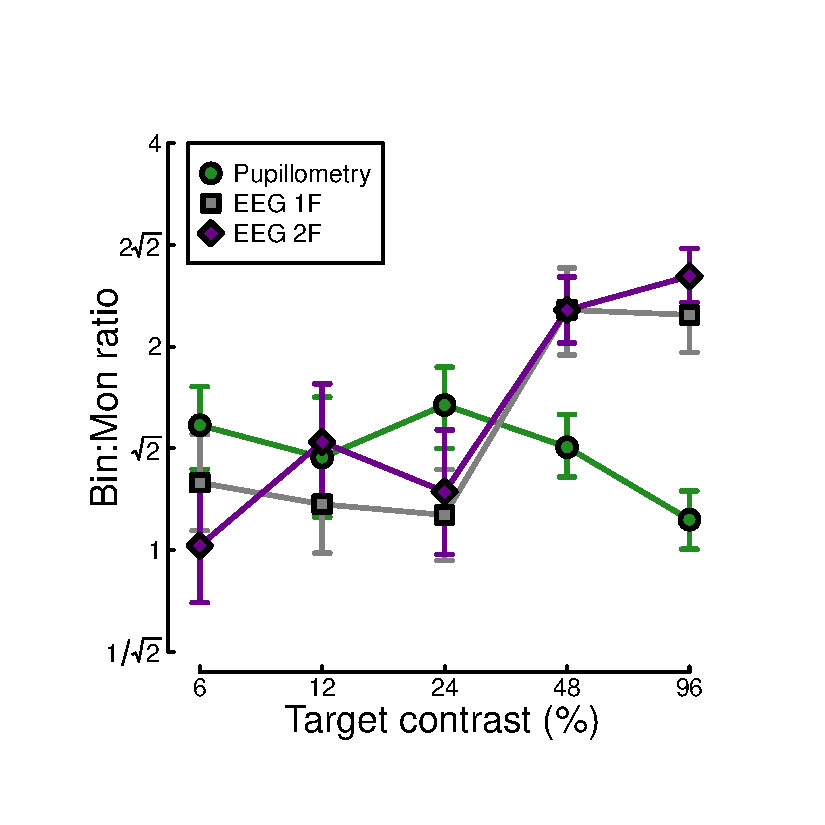
\includegraphics[width=0.5\linewidth]{Figures/BSratios} 

}

\caption{Ratio of binocular to monocular response for three data types. Each ratio is the average of ratios for N=30 participants, and error bars indicate bootstrapped standard errors.}\label{fig:BSratios}
\end{figure}

\hypertarget{experiment-2}{%
\subsection{Experiment 2}\label{experiment-2}}

The strong binocular facilitation and weak interocular suppression in the EEG data from Experiment 1 was very different from previous findings on binocular combination using steady-state EEG with grating stimuli (Baker and Wade, 2017). One possible explanation is that the lower temporal frequency used here (2Hz, vs 5 or 7Hz in previous work) might be responsible for this difference. We therefore ran a second experiment to compare monocular and binocular responses at a range of temporal frequencies. Only EEG data were collected for this experiment, as the pupil response is negligible above around 2Hz (Spitschan et al., 2014).

Results from the temporal frequency experiment are shown in \ref{fig:TFdata}. Figure \ref{fig:TFdata}a shows the Fourier spectra for responses to binocular flicker at 5 different frequencies (2, 4, 8, 16, and 30 Hz). From 2 to 16 Hz, clear signals are observed at each fundamental frequency, and typically also their higher harmonics (integer multiples of the fundamental). However, at 30 Hz (upper row), the responses recorded were not demonstrably above the noise baseline. Figure \ref{fig:TFdata}b compares the monocular and binocular responses at each stimulation frequency. Here we replicate the substantial summation effect across frequencies up to and including 16Hz (Fig. \ref{fig:TFdata}c), demonstrating that strong binocular facilitation in the EEG data of Experiment 1 cannot be attributed to our use of 2Hz flicker.

\begin{figure}

{\centering 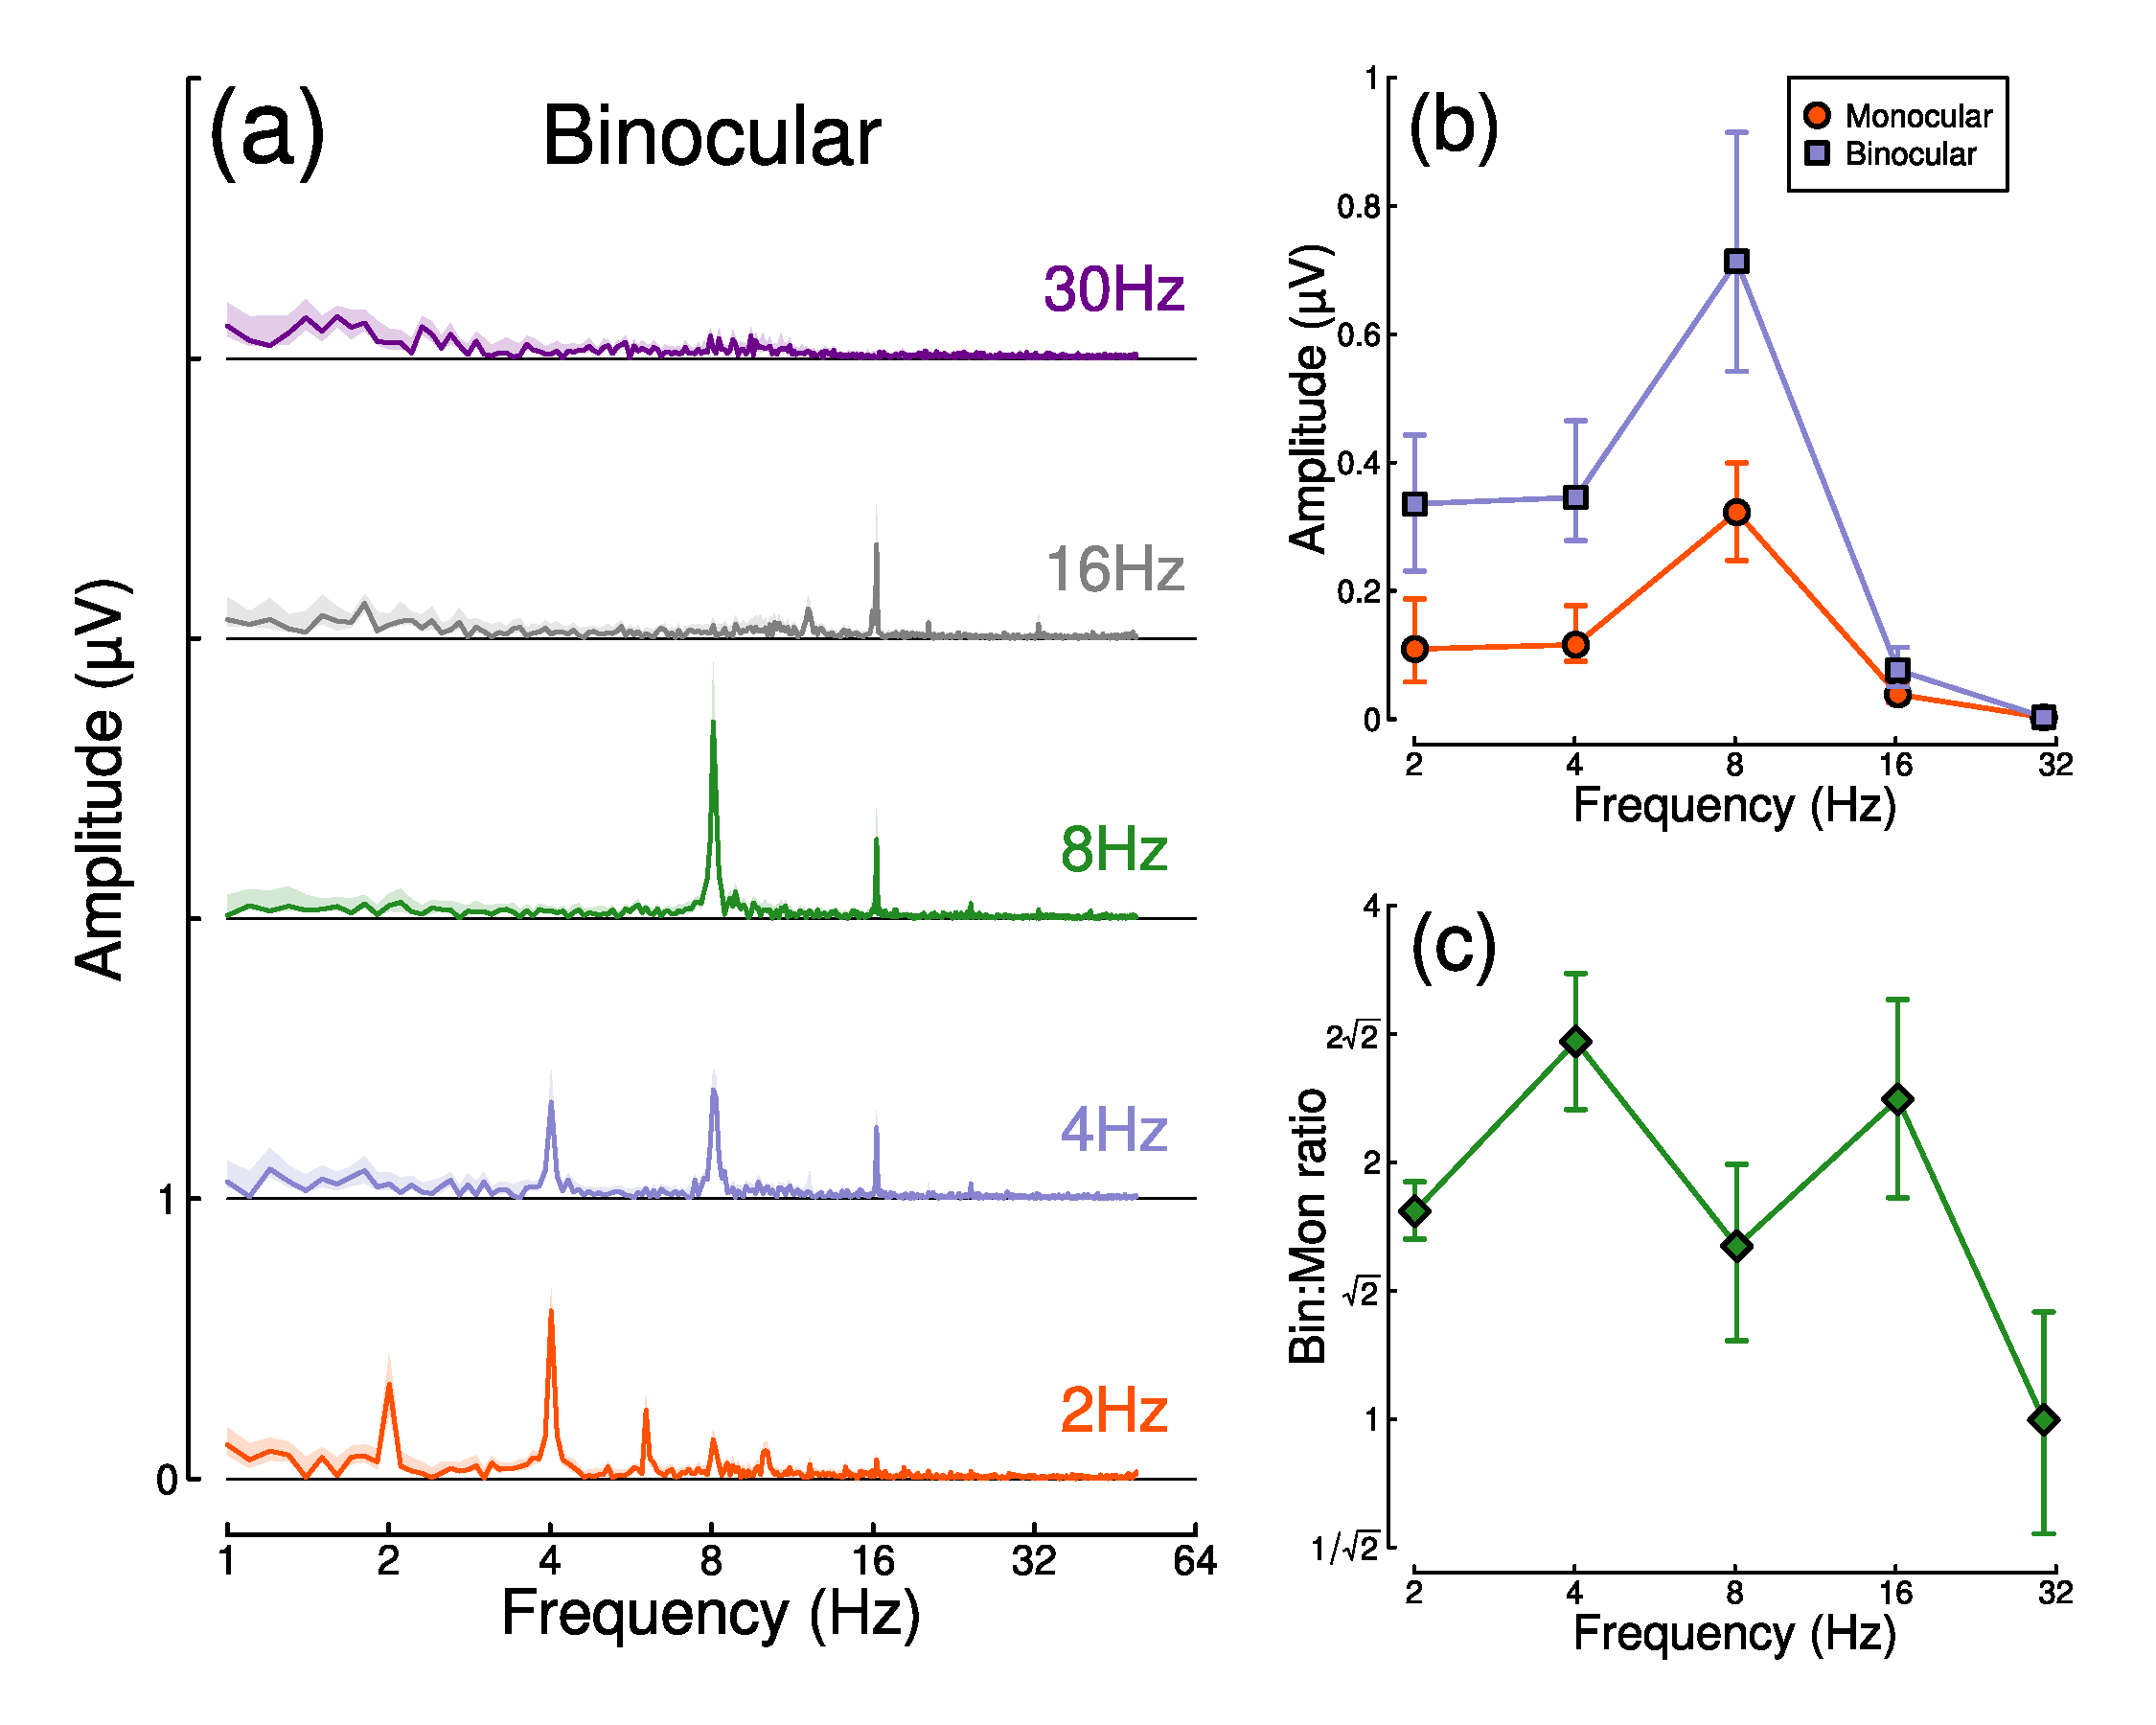
\includegraphics{Figures/TFdata} 

}

\caption{Binocular facilitation at different temporal frequencies. Panel (a) shows Fourier spectra for responses to binocular flicker at 5 different frequencies (offset vertically for clarity). Panel (b) shows the response at each stimulation frequency for monocular (red circles) and binocular (blue squares) presentation. Panel (c) shows the ratio of binocular to monocular responses. Error bars and shaded regions indicate bootstrapped standard errors across N=12 participants.}\label{fig:TFdata}
\end{figure}

\hypertarget{experiment-3}{%
\subsection{Experiment 3}\label{experiment-3}}

In Experiment 1 we found evidence of much stronger binocular facilitation for cortical responses to luminance flicker (measured using EEG), compared with subcortical responses (measured using pupillometry). Since perception is dependent on cortical responses, these results provide a clear prediction for percieved contrast judgements indexed by psychophysical contrast matching paradigms (e.g. Anstis and Ho, 1998; Levelt, 1965; Quaia et al., 2018). We therefore conducted such an experiment, in which participants judged which of two stimuli had the greater perceived amplitude of flicker. One stimulus was a matching stimulus, that had a fixed binocular flicker amplitude of either 24\% or 48\% (temporal) contrast. The other stimulus was a target stimulus, the contrast of which was controlled by a staircase algorithm. We tested 9 ratios of contrast between the left and right eyes.

The results from the matching experiment are shown in Figure \ref{fig:matchingdata}. Each data point indicates the contrast levels required in each eye that were perceptually equivalent to the binocular 24\% (red circles) and 48\% (blue circles) matching contrasts. At both matching contrasts, we see a very substantial increase in the physical contrast required for a monocular target (data points along the x- and y-axes), compared to a binocular target (points along the diagonal of x=y). For example with a 48\% match, the monocular targets required contrasts close to 100\%, whereas binocular targets required a contrast of around 50\%. The data points between these extremes also fall close to the predictions of a linear summation model (diagonal dotted lines), and are inconsistent with a winner-takes-all (or MAX) model (dashed lines). Overall, these matching results are consistent with the approximately linear summation effects observed in the EEG data of Experiment 1 (Figure \ref{fig:EEGdata}c,f).

\begin{figure}

{\centering 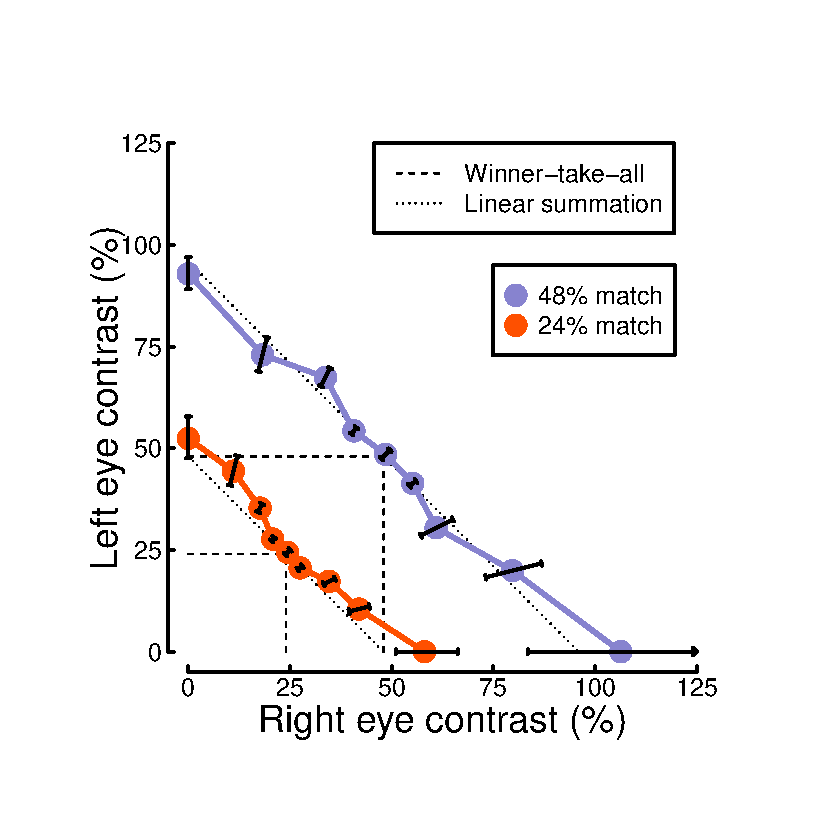
\includegraphics[width=0.5\linewidth]{Figures/matchingdata} 

}

\caption{Contrast matching functions. Dotted and dashed lines are predictions of canonical summation models with a linear exponent (dotted) or an infinite exponent (dashed). Error bars indicate the standard error across participants (N=10), and are constrained along radial lines converging at the origin.}\label{fig:matchingdata}
\end{figure}

\hypertarget{computational-modelling}{%
\subsection{Computational modelling}\label{computational-modelling}}

We fitted a computational model to the data from Experiments 1 \& 3 using a hierarchical Bayesian approach. The model behaviour is displayed in Figure \ref{fig:modelfigure}e-h, with empirical data replotted in Figure \ref{fig:modelfigure}a-d for comparison. In general, the model captures the key characteristics of the empirical data. Note that there are some minor discrepancies, which are a consequence of the hierarchical nature of the modelling. In brief, the model is fitted to the amplitudes for each participant, and group-level parameter estimates are derived based on these fits (see Table \ref{tab:paramtable}). This procedure discards the phase information, whereas the empirical averages are coherently averaged across participants (retaining phase information). This explains the amplitude differences between model and data, particularly at low target contrast levels, but are of no consequence for the pattern of relative responses across conditions.

We were particularly interested in comparing the weight of interocular suppression across data sets. We therefore plot the posterior distributions for this parameter for all four data sets (see Figure \ref{fig:modelfigure}i). The key finding is that the pupillometry results (green distribution) display a much greater weight of interocular suppression compared with the other data sets (grey, purple and yellow distributions). There is no overlap between the pupillometry distribution and any of the other three. All four distributions are also meaningfully below a weight of 1 -- the value that previous work using grating stimuli would predict (Baker and Wade, 2017; Meese et al., 2006). These results offer an explanation of the empirical data: the strong interocular suppression for the pupillometry data is consistent with the weak binocular facilitation, and measurable dichoptic masking observed using that method. The weaker suppression for the other experiments is consistent with the near-linear binocular facilitation effects, and absence of dichoptic masking.

\begin{figure}

{\centering 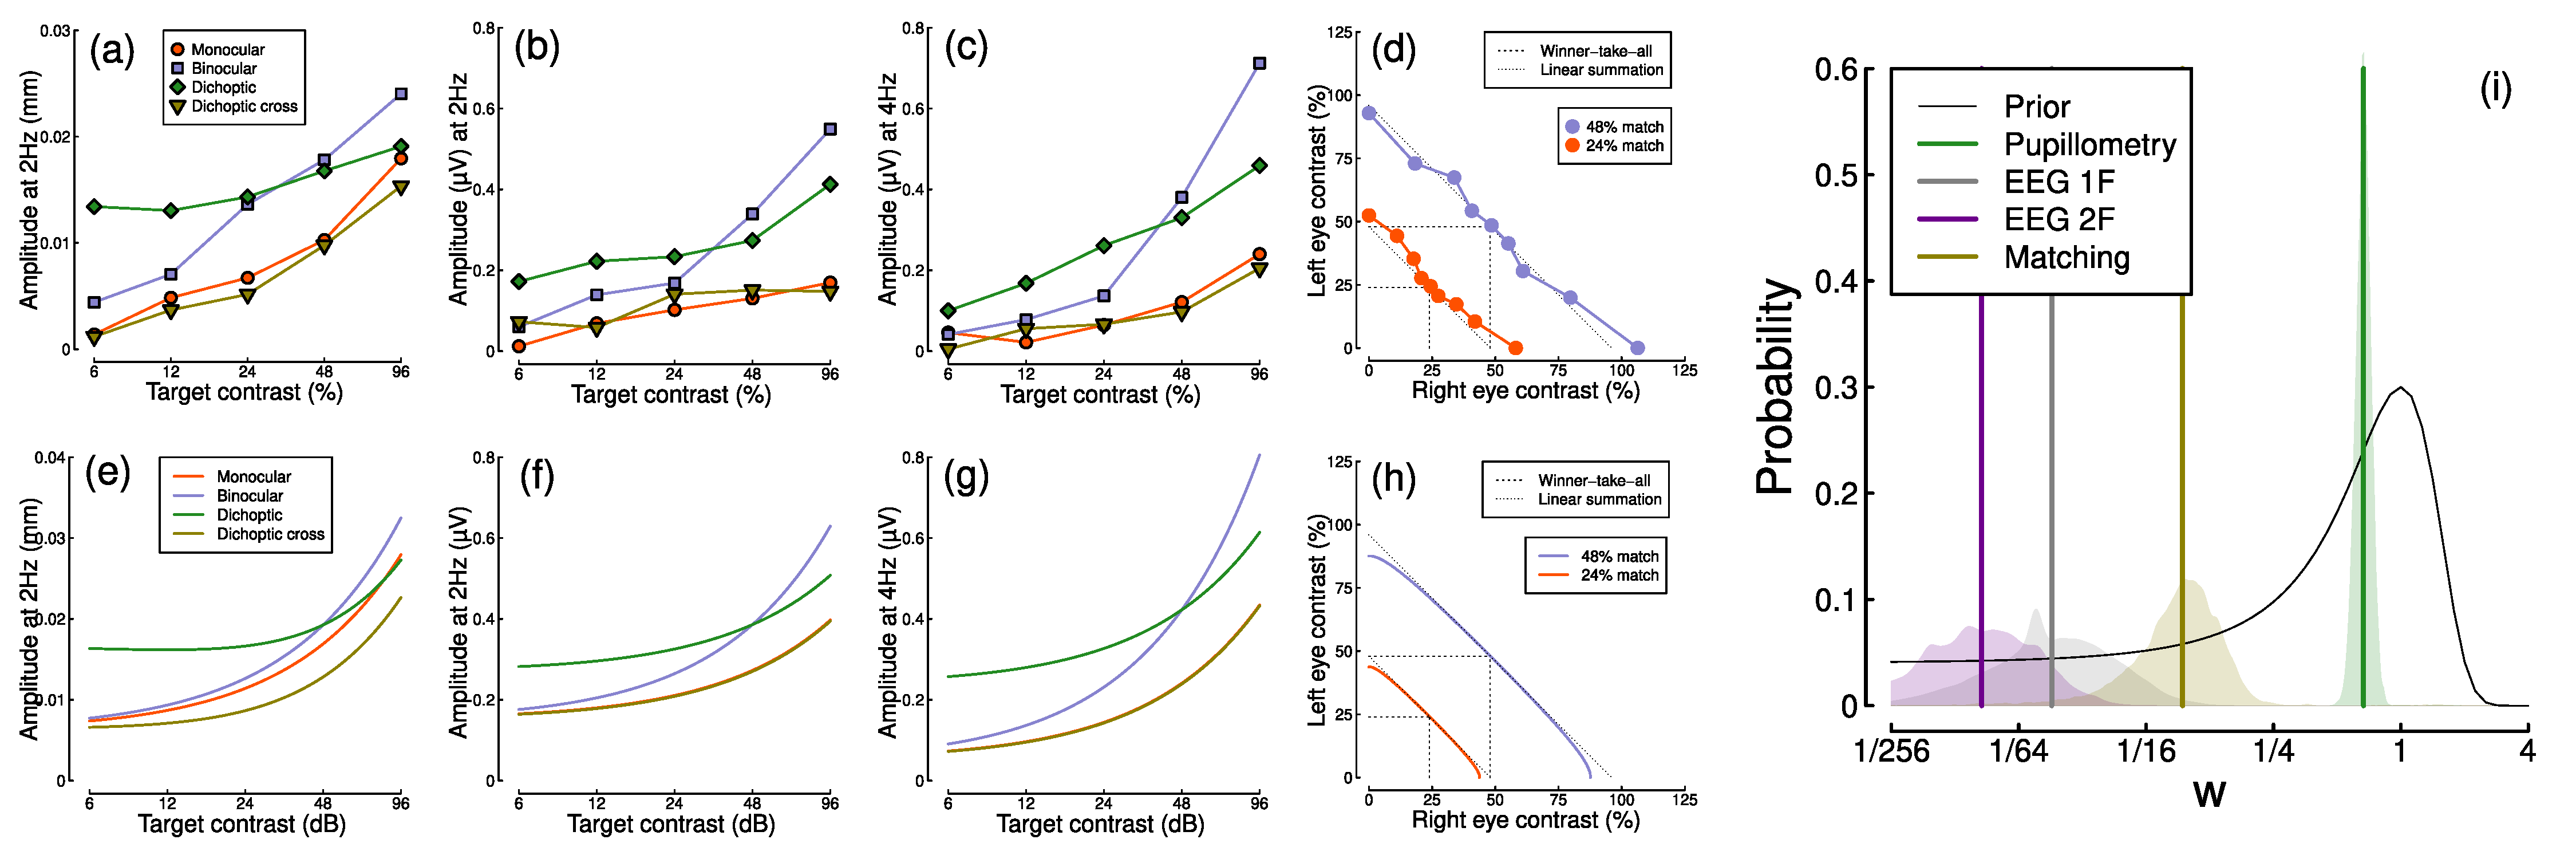
\includegraphics{Figures/modelfigure} 

}

\caption{Summary of computational modelling. Panels (a-d) show empirical data from key conditions, replotted from earlier figures for the pupillometry (a), first harmonic EEG responses (b), second harmonic EEG responses (c) and contrast matching (d) experiments. Panels (e-h) show model behaviour for the same conditions, generated using the median group-level parameter values.  Panel (i) shows the posterior probability distributions of the interocular suppression parameter for each of the four model fits. The pupillometry distribution (green) is centred about a substantially higher suppressive weight than for the other data types (note the logarithmic x-axis). The black curve shows the (scaled) prior distribution for the weight parameter.}\label{fig:modelfigure}
\end{figure}

\begin{table}

\caption{\label{tab:paramtable}Summary of median parameter values.}
\centering
\begin{tabular}[t]{l|c|c|c|c}
\hline
Data set & Z & k & w & Rmax\\
\hline
Pupillometry & 2.37 & 0.01 & 0.67 & 0.00023\\
\hline
EEG 1F & 2.59 & 0.15 & 0.02 & 0.0026\\
\hline
EEG 2F & 2.21 & 0.06 & 0.01 & 0.00404\\
\hline
Matching & 0.30 & 5.07 & 0.09 & -\\
\hline
\end{tabular}
\end{table}

\hypertarget{discussion}{%
\section{Discussion}\label{discussion}}

\hypertarget{references}{%
\section*{References}\label{references}}
\addcontentsline{toc}{section}{References}

\hypertarget{refs}{}
\begin{CSLReferences}{1}{0}
\leavevmode\vadjust pre{\hypertarget{ref-Anderson1989}{}}%
Anderson PA, Movshon JA. 1989. Binocular combination of contrast signals. \emph{Vision Res} \textbf{29}:1115--32. doi:\href{https://doi.org/10.1016/0042-6989(89)90060-6}{10.1016/0042-6989(89)90060-6}

\leavevmode\vadjust pre{\hypertarget{ref-Angee2021}{}}%
Angée C, Nedelec B, Erjavec E, Rozet J-M, Fares Taie L. 2021. Congenital microcoria: Clinical features and molecular genetics. \emph{Genes (Basel)} \textbf{12}. doi:\href{https://doi.org/10.3390/genes12050624}{10.3390/genes12050624}

\leavevmode\vadjust pre{\hypertarget{ref-Anstis1998}{}}%
Anstis S, Ho A. 1998. Nonlinear combination of luminance excursions during flicker, simultaneous contrast, afterimages and binocular fusion. \emph{Vision Res} \textbf{38}:523--39. doi:\href{https://doi.org/10.1016/s0042-6989(97)00167-3}{10.1016/s0042-6989(97)00167-3}

\leavevmode\vadjust pre{\hypertarget{ref-Baker2021}{}}%
Baker DH. 2021. Statistical analysis of periodic data in neuroscience. \emph{Neurons, Behavior, Data analysis, and Theory} \textbf{5}. doi:\href{https://doi.org/10.51628/001c.27680}{10.51628/001c.27680}

\leavevmode\vadjust pre{\hypertarget{ref-Baker2018}{}}%
Baker DH, Lygo FA, Meese TS, Georgeson MA. 2018. Binocular summation revisited: Beyond \(\sqrt{2}\). \emph{Psychol Bull} \textbf{144}:1186--1199. doi:\href{https://doi.org/10.1037/bul0000163}{10.1037/bul0000163}

\leavevmode\vadjust pre{\hypertarget{ref-Baker2020}{}}%
Baker DH, Vilidaite G, McClarnon E, Valkova E, Bruno A, Millman RE. 2020. Binaural summation of amplitude modulation involves weak interaural suppression. \emph{Sci Rep} \textbf{10}:3560. doi:\href{https://doi.org/10.1038/s41598-020-60602-5}{10.1038/s41598-020-60602-5}

\leavevmode\vadjust pre{\hypertarget{ref-Baker2017}{}}%
Baker DH, Wade AR. 2017. Evidence for an optimal algorithm underlying signal combination in human visual cortex. \emph{Cereb Cortex} \textbf{27}:254--264. doi:\href{https://doi.org/10.1093/cercor/bhw395}{10.1093/cercor/bhw395}

\leavevmode\vadjust pre{\hypertarget{ref-Baker2012}{}}%
Baker DH, Wallis SA, Georgeson MA, Meese TS. 2012. Nonlinearities in the binocular combination of luminance and contrast. \emph{Vision Res} \textbf{56}:1--9. doi:\href{https://doi.org/10.1016/j.visres.2012.01.008}{10.1016/j.visres.2012.01.008}

\leavevmode\vadjust pre{\hypertarget{ref-Campbell1965}{}}%
Campbell FW, Green DG. 1965. Monocular versus binocular visual acuity. \emph{Nature} \textbf{208}:191--2. doi:\href{https://doi.org/10.1038/208191a0}{10.1038/208191a0}

\leavevmode\vadjust pre{\hypertarget{ref-Carpenter2017}{}}%
Carpenter B, Gelman A, Hoffman MD, Lee D, Goodrich B, Betancourt M, Brubaker M, Guo J, Li P, Riddell A. 2017. Stan: A probabilistic programming language. \emph{Journal of Statistical Software, Articles} \textbf{76}:1--32. doi:\href{https://doi.org/10.18637/jss.v076.i01}{10.18637/jss.v076.i01}

\leavevmode\vadjust pre{\hypertarget{ref-Delorme2004}{}}%
Delorme A, Makeig S. 2004. {EEGLAB}: An open source toolbox for analysis of single-trial {EEG} dynamics including independent component analysis. \emph{J Neurosci Methods} \textbf{134}:9--21. doi:\href{https://doi.org/10.1016/j.jneumeth.2003.10.009}{10.1016/j.jneumeth.2003.10.009}

\leavevmode\vadjust pre{\hypertarget{ref-Ding2006}{}}%
Ding J, Sperling G. 2006. A gain-control theory of binocular combination. \emph{Proc Natl Acad Sci U S A} \textbf{103}:1141--6. doi:\href{https://doi.org/10.1073/pnas.0509629103}{10.1073/pnas.0509629103}

\leavevmode\vadjust pre{\hypertarget{ref-Figueira2022}{}}%
Figueira JSB, Kutlu E, Scott LS, Keil A. 2022. The FreqTag toolbox: A principled approach to analyzing electrophysiological time series in frequency tagging paradigms. \emph{Dev Cogn Neurosci} \textbf{54}:101066. doi:\href{https://doi.org/10.1016/j.dcn.2022.101066}{10.1016/j.dcn.2022.101066}

\leavevmode\vadjust pre{\hypertarget{ref-Kassner2014}{}}%
Kassner M, Patera W, Bulling A. 2014. Pupil: An open source platform for pervasive eye tracking and mobile gaze-based interactionProceedings of the 2014 {ACM} International Joint Conference on Pervasive and Ubiquitous Computing: Adjunct Publication. UbiComp '14 Adjunct; {ACM}. pp. 1151--1160. doi:\href{https://doi.org/10.1145/2638728.2641695}{10.1145/2638728.2641695}

\leavevmode\vadjust pre{\hypertarget{ref-Kingdom2015}{}}%
Kingdom FAA, Libenson L. 2015. Dichoptic color saturation mixture: Binocular luminance contrast promotes perceptual averaging. \emph{J Vis} \textbf{15(5)}:2. doi:\href{https://doi.org/10.1167/15.5.2}{10.1167/15.5.2}

\leavevmode\vadjust pre{\hypertarget{ref-Legge1984}{}}%
Legge GE. 1984. Binocular contrast summation--II. Quadratic summation. \emph{Vision Res} \textbf{24}:385--94. doi:\href{https://doi.org/10.1016/0042-6989(84)90064-6}{10.1016/0042-6989(84)90064-6}

\leavevmode\vadjust pre{\hypertarget{ref-Levelt1965}{}}%
Levelt WJ. 1965. Binocular brightness averaging and contour information. \emph{Br J Psychol} \textbf{56}:1--13. doi:\href{https://doi.org/10.1111/j.2044-8295.1965.tb00939.x}{10.1111/j.2044-8295.1965.tb00939.x}

\leavevmode\vadjust pre{\hypertarget{ref-Mathot2018}{}}%
Mathôt S. 2018. Pupillometry: Psychology, physiology, and function. \emph{J Cogn} \textbf{1}:16. doi:\href{https://doi.org/10.5334/joc.18}{10.5334/joc.18}

\leavevmode\vadjust pre{\hypertarget{ref-McDougal2010}{}}%
McDougal DH, Gamlin PD. 2010. The influence of intrinsically-photosensitive retinal ganglion cells on the spectral sensitivity and response dynamics of the human pupillary light reflex. \emph{Vision Res} \textbf{50}:72--87. doi:\href{https://doi.org/10.1016/j.visres.2009.10.012}{10.1016/j.visres.2009.10.012}

\leavevmode\vadjust pre{\hypertarget{ref-Meese2006}{}}%
Meese TS, Georgeson MA, Baker DH. 2006. Binocular contrast vision at and above threshold. \emph{J Vis} \textbf{6}:1224--43. doi:\href{https://doi.org/10.1167/6.11.7}{10.1167/6.11.7}

\leavevmode\vadjust pre{\hypertarget{ref-Purves2008}{}}%
Purves D, Brannon EM, Cabeza R, LaBar KS, Huettel SA, Platt ML, Woldorff MG. 2008. Principles of {Cognitive} {Neuroscience}. Oxford University Press, Incorporated.

\leavevmode\vadjust pre{\hypertarget{ref-Quaia2018}{}}%
Quaia C, Optican LM, Cumming BG. 2018. Binocular summation for reflexive eye movements. \emph{J Vis} \textbf{18}:7. doi:\href{https://doi.org/10.1167/18.4.7}{10.1167/18.4.7}

\leavevmode\vadjust pre{\hypertarget{ref-Schrodinger1926}{}}%
Schrödinger E. 1926. Die gesichtsempfindungen.Mueller-Pouillets Lehrbuch Der Physik (11th Ed.). Vieweg: Braunschweig. pp. 456--560.

\leavevmode\vadjust pre{\hypertarget{ref-Spitschan2014}{}}%
Spitschan M, Jain S, Brainard DH, Aguirre GK. 2014. Opponent melanopsin and s-cone signals in the human pupillary light response. \emph{Proc Natl Acad Sci U S A} \textbf{111}:15568--72. doi:\href{https://doi.org/10.1073/pnas.1400942111}{10.1073/pnas.1400942111}

\leavevmode\vadjust pre{\hypertarget{ref-Victor1991}{}}%
Victor JD, Mast J. 1991. A new statistic for steady-state evoked potentials. \emph{Electroencephalogr Clin Neurophysiol} \textbf{78}:378--88. doi:\href{https://doi.org/10.1016/0013-4694(91)90099-p}{10.1016/0013-4694(91)90099-p}

\leavevmode\vadjust pre{\hypertarget{ref-Wang2015}{}}%
Wang C-A, Munoz DP. 2015. A circuit for pupil orienting responses: Implications for cognitive modulation of pupil size. \emph{Curr Opin Neurobiol} \textbf{33}:134--40. doi:\href{https://doi.org/10.1016/j.conb.2015.03.018}{10.1016/j.conb.2015.03.018}

\leavevmode\vadjust pre{\hypertarget{ref-Wyatt1981}{}}%
Wyatt HJ, Musselman JF. 1981. Pupillary light reflex in humans: Evidence for an unbalanced pathway from nasal retina, and for signal cancellation in brainstem. \emph{Vision Res} \textbf{21}:513--25. doi:\href{https://doi.org/10.1016/0042-6989(81)90097-3}{10.1016/0042-6989(81)90097-3}

\end{CSLReferences}

\end{document}
